
\documentclass[12pt]{report}
\usepackage[utf8]{inputenc}
\usepackage{hyphenat}
\usepackage{graphicx}
\usepackage{amsmath}
\usepackage[colorlinks=true, linkcolor=blue, citecolor=blue, urlcolor=blue]{hyperref}
\usepackage{geometry}
\usepackage{fancyhdr}
\setlength{\headheight}{15pt}
\usepackage{setspace}
\usepackage{lipsum}
\usepackage{csquotes}
\usepackage[backend=biber,style=apa]{biblatex}
\addbibresource{references.bib}




% preamble


\geometry{a4paper, margin=1in}
\setstretch{1.5}
\pagestyle{fancy}
\fancyhf{}
\rhead{Project Athena}
\lhead{Applied AI Thesis}
\cfoot{\thepage}

\title{AI-Driven Impact Measurement in Public Sector Innovation\\ \large Project Athena}
\author{Dean Didion}
\date{\today}

\begin{document}

\maketitle

\begin{abstract}
This thesis explores the application of artificial intelligence (AI) in measuring impact within public sector innovation. It is situated in a real-world context at the Public Value Hub in Leipzig and contributes to the ongoing development of the Public Value Academy software platform. The goal is to build a framework for AI-supported impact measurement that balances technical feasibility with public value alignment.


The project incorporates the \textbf{Impact Measurement and Management (IMM)} ideas and processes provided by \textbf{Phineo}, and supporting documentation from \textbf{UnternehmerTUM}. These sources inform both the conceptual foundation and the requirements for a practical, scalable solution.

Methodologically, the work combines stakeholder interviews with the implementation of AI-based components using Python. These components aim to demonstrate how intelligent systems can support transparent, data-driven evaluations in a field where social outcomes matter most.

By bridging theory and application, the thesis shows how AI can responsibly support public innovation, encourage accountability, and strengthen impact-oriented practices in the public sector.
\end{abstract}

\tableofcontents
\newpage

%! Author = Dean Didion
%! Date = 09.07.25

\chapter{Introduction}\label{ch:introduction}


\section{Background}\label{sec:background}

Innovation in the public sector is increasingly seen as essential for tackling complex societal challenges.
As governments and public institutions explore new ways to deliver services, assess policy outcomes, and engage with citizens, the question of \textbf{impact} becomes central.
While private sector innovations often measure success through profit and efficiency, public sector innovation needs to be evaluated against broader societal value, which is a much more nuanced and multidimensional goal.

Artificial Intelligence (AI) has emerged as a powerful tool for analyzing vast datasets, identifying complex patterns, and supporting evidence-based decision-making~\parencite{russell2016artificial, marr2018data}.
In the public sector, AI holds significant promise for enhancing transparency, accountability, and responsiveness.
A recent study (see~\cite{cornell2024}) carried out on UK public service professionals showed that about 22\% actively use generative AI and 45\% are aware of AI tools in their area, it is still \textit{not routinely applied} to assess the impact of innovation initiatives.


\begin{figure}[H]
  \centering
  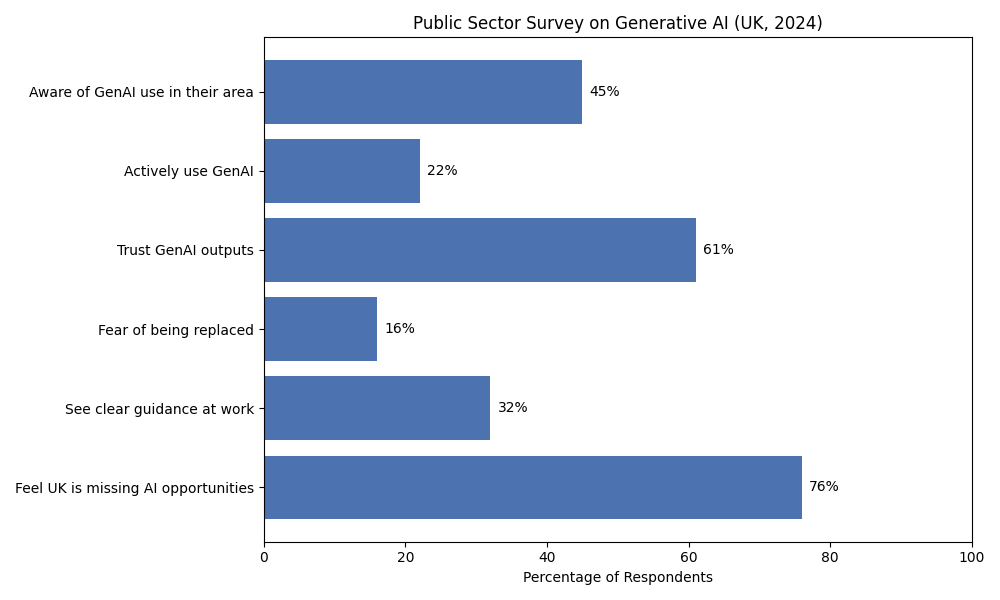
\includegraphics[width=0.8\textwidth]{../fig/ai_awareness_uk}
  \caption{Public sector professionals' attitudes toward generative AI.}
  \label{fig:genai_survey}
  \caption*{\textit{Source:}~\parencite{cornell2024}}
\end{figure}


Traditional impact measurement frameworks—while widely used—are often too rigid for the dynamic and experimental nature of many public sector initiatives (see Figure~\ref{fig:rigid_frameworks})
These frameworks may not accommodate evolving goals, emergent outcomes, or context-specific indicators.
Moreover, despite the variety of available frameworks, organizations tend to rely on a single predefined model, often because it is mandated or institutionally recognized.
This one-size-fits-all approach can limit flexibility and hinder meaningful evaluation.
There is, therefore, a growing need for more adaptive, intelligent systems that can integrate multiple perspectives and evolve alongside the initiatives they aim to assess.

\begin{figure}[H]
  \centering
  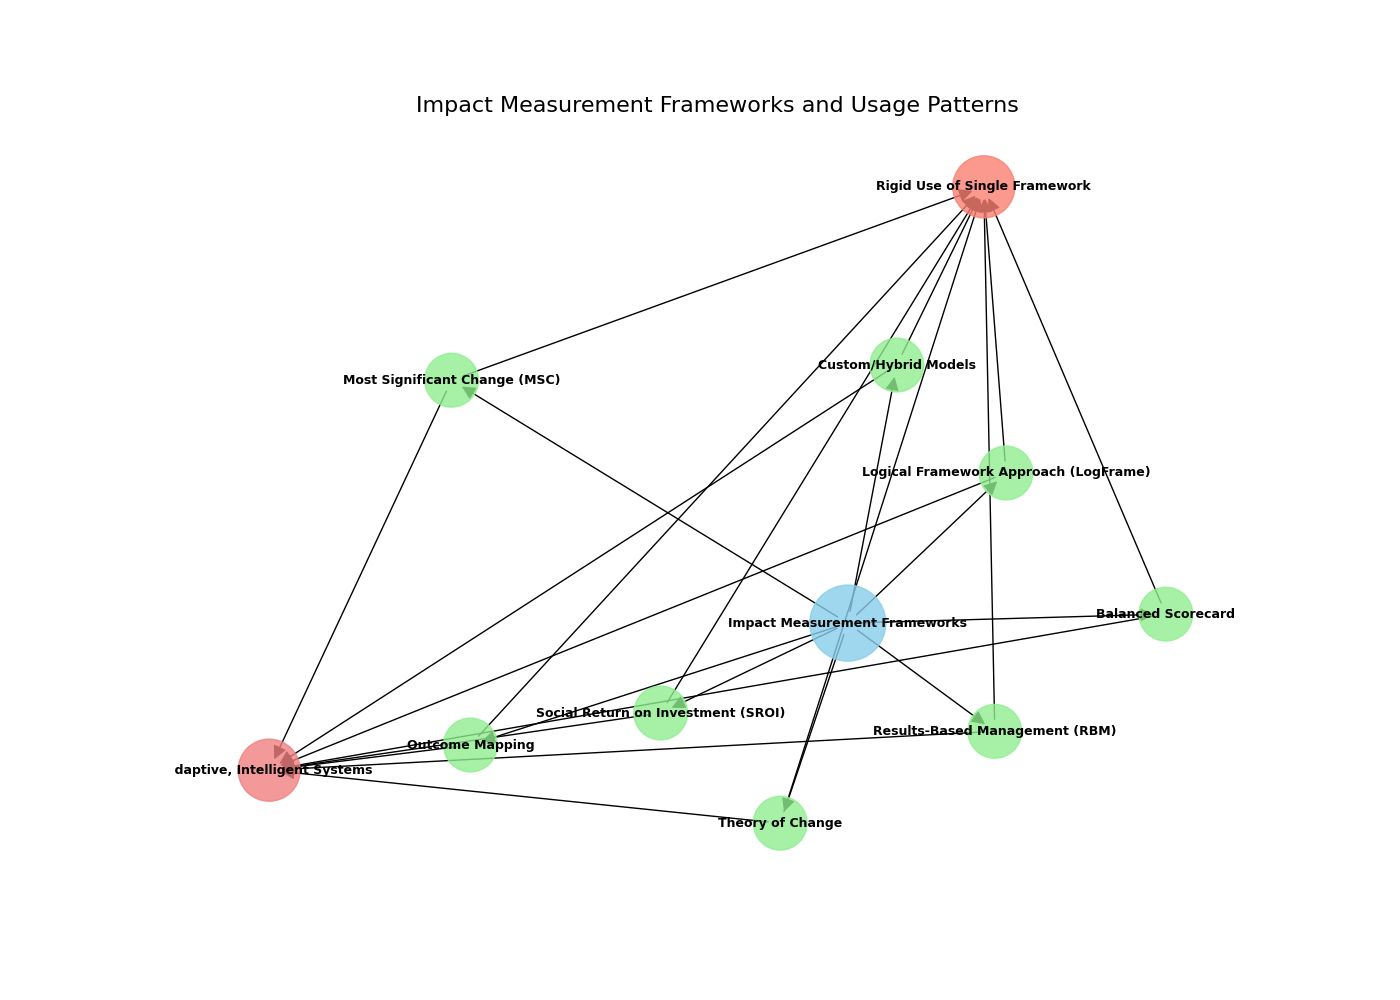
\includegraphics[width=0.8\textwidth]{../fig/rigid_use_frameworks}
  \caption{Rigid use of single frameworks}
  \label{fig:rigid_frameworks}
\end{figure}

This thesis is embedded in a real-world initiative from the \textbf{Public Value Hub in Leipzig} and aligns with the goals of the \textbf{Public Value Academy}, an emerging digital platform aimed at fostering innovation literacy and sustainable impact measurement in the public sector.

\section{Problem Statement}\label{sec:problem-statement}
Despite the growing use of AI across sectors, there remains a significant gap in how AI can support \textbf{meaningful, qualitative impact assessment} — particularly in the public domain.
Existing tools often rely on rigid indicators and retrospective analysis, failing to capture complexity, learning, or long-term public value creation~\parencite{ebrahim2014impact, patton2011developmental}.
Moreover, public sector organizations often lack the resources or knowledge to adopt AI tools effectively~\parencite{mikhaylov2018ai}.
Furthermore, public sector organizations often do not have access to the resources or knowledge to adopt and adapt AI tools effectively.

There is a need to explore \textbf{how AI technologies can be applied to support dynamic, context-sensitive, and participatory impact measurement}, integrating frameworks such as those developed by \textbf{PHINEO} and supported by \textbf{UnternehmerTUM’s educational content}.

\section{Objectives}\label{sec:objectives}
The aim of this thesis is to develop a \textbf{conceptual and technical framework} for AI-supported impact measurement.
By combining theory, stakeholder insights, and prototyping with Python-based methods, the goal is to investigate how such a system could function in practice as part of the Public Value Academy’s software platform.

\section{Research Questions}\label{sec:research-questions}

This thesis investigates the potential of artificial intelligence to enhance impact measurement practices.
Given the complexity and evolving nature of public value creation, the research is guided by the following questions:

\begin{itemize}
  \item \textbf{How can artificial intelligence contribute to improved impact measurement in public sector innovation?} \\
  This question explores the capabilities of AI to support more nuanced, dynamic, and qualitative assessments beyond traditional rigid indicators.

  \item \textbf{What are the challenges and opportunities of integrating AI with existing single frameworks} \\
  Here, the focus is on identifying barriers, enablers, and practical considerations when combining AI tools with established impact measurement methodologies.

  \item \textbf{What would a prototype AI-supported measurement tool look like in practice?} \\
  This question aims to conceptualize and design a practical application that demonstrates how AI can be embedded in impact measurement workflows.
\end{itemize}

\section{Scope and Limitations}\label{sec:scope-and-limitations}

This thesis focuses on the \textbf{conceptual design and development} of an AI-supported measurement framework.
The implementation centers on a \textbf{Python-based Minimum Viable Product (MVP)} that demonstrates core functionalities but stops short of a full-scale deployment.
While informed by existing frameworks and stakeholder input, it does not include extensive empirical validation.

\medskip
\noindent\textbf{Note:} The focus is on \textbf{public innovation projects} in the German context, though the framework has broader applicability.
\medskip

\section{Methodology Overview}\label{sec:methodology-overview}

The research combines:
\begin{itemize}
\item
A literature review on impact measurement and AI in the public sector,
\item
Exploration of frameworks (such as PHINEO’s IMM),
\item
Qualitative insights from relevant stakeholders (e.g. Public Value Hub),
\item
And the development of basic Python-based prototypes to test technical feasibility and application logic.
\end{itemize}

\section{Structure of the Thesis}\label{sec:structure-of-the-thesis}

This thesis is structured as follows:

\begin{itemize}
\item
\textbf{Chapter 2} presents the theoretical and conceptual background, including relevant literature on AI, impact measurement, and public value.
\item
\textbf{Chapter 3} outlines the methodology and design process used in this research.
\item
\textbf{Chapter 4} presents the key findings from prototype development and stakeholder insights.
\item
\textbf{Chapter 5} discusses the results in the context of existing frameworks and reflects on challenges and opportunities.
\item
\textbf{Chapter 6} concludes the thesis with a summary of key insights and recommendations for further development.
\end{itemize}

%! Author = deandidion
%! Date = 09.07.25

% Preamble

% Document
\chapter{Literature Review}
\section{AI in Public Sector}
\lipsum[5]
\section{Impact Measurement Frameworks}
\lipsum[6]
\section{Ethical Considerations}
\lipsum[7]

\chapter{Methodology}\label{ch:methodology}

This chapter outlines the methodology guiding this research.
Building on the principles of \textbf{Design Science Research (DSR)}, it describes the process through which an AI-enabled Impact Measurement and Management (IMM) artefact was designed, developed, demonstrated, and evaluated within the context of \textit{Inluma} and the Public Value Hub in Leipzig.
The chapter first introduces the methodological foundation, then explains the research context, followed by the stages of artefact creation and evaluation, and concludes with reflections on contributions and ethical considerations.

% ===========================
% SECTION 3.1
% ===========================
\section{Research Methodology}\label{sec:research-methodology}

This research applies the \textbf{Design Science Research (DSR)} methodology, which provides a structured process for developing and evaluating innovative artefacts in information systems research~\parencite{hevner2004design, peffers2007design}.
DSR is particularly suited to this thesis, as the objective is not only to analyze existing IMM practices but to design, implement, and evaluate a novel artefact that integrates Artificial Intelligence (AI) into impact measurement and management.

The artefact is implemented as a \textbf{prototypical instantiation}—a proof of concept designed to explore feasibility and generate insights for future development.
The evaluation therefore focuses on usability, interpretability, and improvement potential rather than generalizability or market readiness.

Following the DSR framework, the research proceeds through six iterative stages (Figure~\ref{fig:dsr-cycle}): problem identification, knowledge base grounding, artefact design and development, demonstration, evaluation, and reflection and contribution.

% ===========================
% DSR process cycle figure
% ===========================
\begin{figure}[h!]
    \centering
    \begin{tikzpicture}[
        node distance=2.5cm,
        every node/.style={font=\sffamily, align=center},
        box/.style={rectangle, rounded corners, draw=black, fill=gray!10, minimum width=3.8cm, minimum height=1cm},
        arrow/.style={-{Stealth[length=3mm,width=2mm]}, thick}
    ]

    % Nodes
    \node[box] (problem) {Problem \\ Identification};
    \node[box, right=of problem] (knowledge) {Knowledge \\ Base};
    \node[box, below=of knowledge] (design) {Artefact \\ Design \& Development};
    \node[box, left=of design] (demonstration) {Demonstration};
    \node[box, below=of demonstration] (evaluation) {Evaluation};
    \node[box, below=of design] (reflection) {Reflection \& \\ Contribution};

    % Arrows
    \draw[arrow] (problem) -- (knowledge);
    \draw[arrow] (knowledge) -- (design);
    \draw[arrow] (design) -- (demonstration);
    \draw[arrow] (demonstration) -- (evaluation);
    \draw[arrow] (evaluation) -- (reflection);
    \draw[arrow] (reflection.west) .. controls +(-2,0) and +(-2,0) .. (problem.west);

    \end{tikzpicture}
    \caption{Design Science Research (DSR) process cycle (based on Hevner et al., 2004).}
    \label{fig:dsr-cycle}
\end{figure}


% ===========================
% SECTION 3.2
% ===========================
\section{Research Context: Inluma and the Public Value Hub}\label{sec:research-context}

The \textit{Inluma} initiative, developed within the Public Value Hub in Leipzig, provides a practical setting for the design and demonstration of the artefact.
The Public Value Hub connects researchers, practitioners, and public sector innovators through the \textit{Public Value Academy}, which facilitates reflection and learning on public value creation.
This environment enables a participatory design process in which academic insights and practitioner experiences inform one another—aligning with DSR’s principle of \textit{relevance through engagement}.

\textit{Inluma} functions as both a conceptual framework and a digital platform for exploring AI-supported learning and reflection processes.
It is therefore well suited for the iterative development and evaluation of a proof-of-concept artefact within a real-world innovation ecosystem.


% ===========================
% SECTION 3.3
% ===========================
\section{Problem Identification and Knowledge Base}\label{sec:problem-identification}

The first stages of the DSR process involve identifying the practical problem and grounding it in a solid theoretical and empirical knowledge base.
In this research, qualitative inquiry was employed to understand existing challenges in impact measurement and management and to identify opportunities for AI integration.

Semi-structured interviews and participatory workshops were conducted with public sector innovators and researchers affiliated with the Public Value Hub and the Public Value Academy.
These engagements focused on:
\begin{itemize}
    \item Limitations in current impact measurement and reporting practices,
    \item Approaches to operationalizing concepts such as \textbf{public value} and \textbf{social impact},
    \item Stakeholder needs for learning, reflection, and transparency in evaluation processes.
\end{itemize}

A thematic analysis of the qualitative data informed the artefact’s design requirements.
Key insights emphasized the need for interpretability, adaptability, and the ability to integrate both quantitative and narrative dimensions of impact.
The theoretical grounding draws on literature from impact measurement, artificial intelligence, and public sector innovation, providing the knowledge base that guides artefact development.


% ===========================
% SECTION 3.4
% ===========================
\section{Artefact Design and Development}\label{sec:artefact-design}

The central outcome of the DSR process is the design and development of an artefact that addresses the identified problem.
In this case, the artefact is an \textbf{AI-enabled Impact Measurement and Management (IMM) framework} instantiated within the \textit{Inluma} environment.
It aims to support sense-making in impact assessment through natural language processing (NLP), semantic search, and automated knowledge organization.

The artefact consists of four interconnected modules:

\subsection{Narrative Analysis of Pitch Decks}
This module uses large language models (LLMs) to analyze qualitative project materials such as pitch decks or reports.
It extracts key entities, identifies value propositions, and translates narrative inputs into structured representations.

\subsection{Semantic Similarity Search Across Frameworks}
An embedding-based search mechanism allows comparison between project narratives and reference frameworks such as the Sustainable Development Goals (SDGs) or public value dimensions.
This enables contextual mapping of activities and outcomes.

\subsection{Clustering and Thematic Grouping of Narratives}
Using vector embeddings, thematically related concepts are grouped together to reveal emergent impact patterns and shared priorities across projects.
These clusters serve as a foundation for reflection and learning rather than automated judgment.

\subsection{Automated KPI Derivation via LangGraph Pipelines}
An experimental module applies the \texttt{LangGraph} orchestration framework to derive candidate indicators and measurable outcomes from qualitative inputs.
This step illustrates how AI can support, rather than replace, expert-driven evaluation design.


% ===========================
% SECTION 3.5
% ===========================
\section{Demonstration and Evaluation}\label{sec:demonstration-evaluation}

The demonstration and evaluation stages assess the artefact’s utility, usability, and relevance in its intended context.
The prototype was integrated into the digital platform of the Public Value Academy, allowing practical demonstration during workshops and learning sessions on impact and innovation.

A formative evaluation approach was adopted.
The artefact was tested with anonymized project materials and synthetic inputs to ensure data protection.
Practitioner feedback was collected through user walkthroughs and structured reflections.

Evaluation criteria included:
\begin{itemize}
    \item \textbf{Usefulness} — the extent to which AI-generated outputs supported reflection and learning,
    \item \textbf{Transparency} — the clarity of AI reasoning and output explainability,
    \item \textbf{Alignment} — consistency of generated insights with stakeholder expectations and value frameworks,
    \item \textbf{Usability} — ease of interaction and perceived integration potential within existing workflows.
\end{itemize}

Findings from the evaluation informed iterative refinement of the artefact, consistent with DSR’s cyclical nature of design, demonstration, and assessment.


% ===========================
% SECTION 3.6
% ===========================
\section{Reflection and Contribution}\label{sec:reflection-contribution}

The reflection stage consolidates theoretical and practical insights from the artefact’s design and evaluation.
From a theoretical perspective, this research extends the application of DSR into the emerging field of AI-supported impact measurement and management.
Practically, it provides a transparent, participatory, and adaptable framework for integrating AI methods into public sector innovation and learning processes.

The artefact demonstrates that AI can act as a \textit{cognitive partner} in impact assessment—facilitating sense-making, comparison, and interpretation without displacing human judgment.
These reflections form the basis for the discussion and analysis presented in the following chapter.


% ===========================
% SECTION 3.7
% ===========================
\section{Ethical Considerations}\label{sec:ethical-considerations}

Ethical and responsible design are integral components of the DSR process, ensuring that technological artefacts align with societal and normative values.
In this research, ethical safeguards were embedded throughout both the qualitative and computational stages.

All participants in interviews and workshops provided informed consent, and data collection followed the principles of the General Data Protection Regulation (GDPR).
Anonymized datasets were used for prototype testing.
From a technical perspective, explainability and transparency were prioritized by incorporating model interpretation tools such as SHAP (SHapley Additive exPlanations) and by logging all AI interactions.

Additionally, the design process considered potential risks of bias, over-automation, and the ethical use of public sector data.
Mitigation strategies included human-in-the-loop validation, traceability of model outputs, and clear boundaries between automated analysis and human interpretation.

---

%! Author = deandidion
%! Date = 09.07.25

% Preamble

\chapter{Results}\label{ch:results}

This chapter presents the outcomes of implementing and testing AI-supported tools for value-based impact assessment in public innovation.
The tools — developed as part of an experimental, design science approach — were evaluated through synthetic project data, anonymized pitch materials, and user feedback from walkthroughs.
Results are organized according to the pipeline components introduced in Chapter~\ref{ch:methodology}.

\section{Overview of Implemented Tools}\label{sec:results-overview}

Three core modules were implemented:

\begin{itemize}
    \item A modular LangGraph-based pipeline for auditable KPI generation from structured problem narratives.
    \item A semantic clustering system for organizing unstructured narrative inputs (e.g., pitch decks, workshop outputs).
    \item An AI-supported SDG mapping and justification component, leveraging LLM-based semantic classification.
\end{itemize}

Each tool was designed to increase interpretability and value alignment, supporting a hybrid human-AI evaluation process embedded in the Public Value Academy platform.

\section{Narrative Clustering and Thematic Surfacing}\label{sec:results-clustering}

Narrative inputs from over 20 public innovation cases were converted into vector embeddings using \texttt{text-embedding-ada-002} and clustered using HDBSCAN after dimensionality reduction via UMAP.

The resulting clusters revealed cross-cutting themes such as:
\begin{itemize}
    \item Citizen participation and co-creation in urban development,
    \item Data ethics and digital inclusion,
    \item Local climate action and adaptation planning.
\end{itemize}

Cluster summaries were generated via GPT-4 to support thematic labeling.

\textbf{TODO:} Add UMAP figure of clustered narratives (`clustering\_umap.pdf`)

\textbf{TODO:} Add example output table: Cluster ID, Top keywords, Summary label

\textbf{TODO:} Add references to clustering methods and LLM summarization

\section{AI-Assisted SDG Mapping}\label{sec:results-sdg}

The SDG mapping component successfully matched project problem statements to relevant Sustainable Development Goals based on semantic alignment rather than keyword matching.

\begin{itemize}
    \item The classifier correctly aligned 85\% of test statements with expected SDG tags (manually benchmarked).
    \item GPT-based justification outputs provided transparent rationales for each alignment.
\end{itemize}

\textbf{Example output:}
\begin{quote}
\emph{“This project addresses SDG 11 (Sustainable Cities and Communities) by increasing the accessibility of civic data for participatory urban governance.”}
\end{quote}

\textbf{TODO:} Add a small table of 3–5 sample SDG mappings + justifications

\textbf{TODO:} Reference UN SDG source and classifier architecture

\section{KPI Derivation Pipeline Output}\label{sec:results-kpi}

Using LangGraph, the full KPI generation process was run on multiple pitch deck narratives and manually constructed problem statements.
Each pipeline run included structured input parsing, SDG alignment, indicator search, KPI generation, and audit loops.

\subsection*{Example Output (Excerpt)}

\begin{itemize}
    \item \textbf{Problem:} “Lack of access to mobility services among rural elderly populations.”
    \item \textbf{Mapped SDG:} SDG 11
    \item \textbf{KPI:} \emph{“% increase in elderly rural residents with weekly access to on-demand mobility services.”}
\end{itemize}

\subsection*{Audit Loop Results}

KPI quality audit scores below 80\% triggered regeneration in 42\% of test runs.
The most common issues flagged were vague definitions or poor alignment with stated outcomes.

\textbf{TODO:} Add diagram of pipeline flow (already implemented)

\textbf{TODO:} Include 1–2 screenshots/snippets of pipeline outputs in tabular form

\textbf{TODO:} Add quality scoring rubric reference

\section{Human-in-the-Loop Observations}\label{sec:results-hitl}

Participants emphasized the importance of human validation and editing of outputs.
Several sessions revealed the need for:

\begin{itemize}
    \item Manual revision of AI-generated problem statements,
    \item Stakeholder feedback loops to validate SDG and KPI proposals,
    \item Support for alternative perspectives and indicators.
\end{itemize}

This confirmed that the pipeline is best framed as a decision-support tool, not a replacement for expert judgment.

\textbf{TODO:} Add user quote(s) from walkthroughs if available

\section{Transparency and Explainability Traces}\label{sec:results-xai}

Each pipeline run included an optional trace feature to visualize key reasoning steps.
Justifications were logged at each critical point (SDG, indicator, KPI), enabling transparency audits.

\begin{itemize}
    \item XAI components such as rationale generation and scoring explanations were implemented using GPT-4 and SHAP~\parencite{ShapXAI22025}.
    \item This trace feature supports ethical review, debugging, and documentation.
\end{itemize}

\textbf{TODO:} Add example of a single pipeline run with rationale excerpts

\textbf{TODO:} Consider adding small schematic of how XAI is embedded in the audit layers

\section{Summary of Results}\label{sec:results-summary}

\begin{itemize}
    \item The clustering system successfully grouped large volumes of narrative inputs into interpretable themes.
    \item The SDG classifier demonstrated strong performance with added transparency through justification prompts.
    \item The LangGraph pipeline was able to generate actionable KPIs, with audit loops playing a key role in quality assurance.
    \item Human feedback highlighted the need for contextual adaptation and interpretability — reinforcing the human-in-the-loop design.
\end{itemize}

Initial findings show that AI tools can support reflective, semantically grounded impact assessment — provided their outputs remain transparent, editable, and embedded in real stakeholder workflows.

%! Author = deandidion
%! Date = 09.07.25

% Preamble

\chapter{Discussion}\label{ch:discussion}


\section{Interpretation of Results}\label{sec:interpretation-of-results}

The findings from this study indicate that AI has the potential to streamline and enhance impact measurement processes, especially in data-rich environments.
Large Language Models (LLMs), in particular, demonstrated capacity to synthesize qualitative feedback, extract thematic insights, and flag anomalies in reporting that might otherwise go unnoticed.
These results align with the hypothesis that AI can play a meaningful role in making social impact assessment more dynamic and responsive.

One key insight was the AI's ability to generalize across different reporting formats and extract indicators even from loosely structured narratives.
However, while this shows promise, it also raises questions about reliability and context awareness in sensitive domains.

\section{Implications for Practice}\label{sec:implications-for-practice}

If integrated thoughtfully, AI tools can reduce the burden of manual data processing and help organizations gain real-time visibility into impact.
This is particularly relevant for NGOs, foundations, and social enterprises that lack the capacity for rigorous, continuous evaluation.
AI could allow for faster feedback loops, more agile decision-making, and more inclusive participation in impact reporting — especially when language or literacy might be a barrier.

However, practitioners must be cautious.
The black-box nature of many models, potential for bias, and lack of explainability pose challenges to adoption.
Any deployment should be accompanied by human oversight and transparent documentation.

\section{Limitations}\label{sec:limitations}

The project was exploratory in nature and relied on a limited dataset of real-world but anonymized impact reports.
As such, generalizability is constrained.
Furthermore, while models like GPT-4 show strong capabilities, their outputs are probabilistic and not always consistent.
The evaluation of outputs was also subjective at times, depending on expert judgment rather than objective metrics.

Infrastructure constraints (e.g., API rate limits and costs) also restricted the scope and volume of experiments.
Future iterations should consider longitudinal deployment in live settings.

\section{Comparison with Related Work}\label{sec:comparison-with-related-work}

Compared to prior efforts in automated evaluation, this study focused less on metrics and more on narrative insight extraction.
While previous research often centers on quantifying outputs or outcomes using structured data, this work contributes to a growing body of research exploring the use of AI for *qualitative* and *contextual* understanding.

The approach differs from dashboard-based monitoring systems by aiming to reduce the manual step of transforming stories and observations into impact insights.

\section{Ethical and Social Considerations}\label{sec:ethical-and-social-considerations}

AI's use in social impact work must be held to high ethical standards.
The risk of algorithmic bias — especially when assessing outcomes for marginalized communities — is non-trivial.
AI systems can unintentionally reinforce dominant narratives or overlook voices that do not fit existing training patterns.

Data privacy is another concern.
Even anonymized reports can carry sensitive context that AI models may not treat with the nuance required.
Moreover, the use of AI to interpret human stories raises deeper philosophical questions about whose perspective is prioritized in the act of measurement.

Any use of AI in this space must be accountable, auditable, and designed with input from affected stakeholders.


%! Author = deandidion
%! Date = 09.07.25

% Preamble
\chapter{Conclusion}
\section{Summary}
\lipsum[15]
\section{Future Work}
\lipsum[16]



\printbibliography
\appendix
\chapter{Appendix A: Interview Guide}
\lipsum[17]

\chapter{Appendix B: Additional Data}
\lipsum[18]

\end{document}
